%% Begin slides template file
\pdfminorversion=4
\documentclass[11pt,t,usepdftitle=false,aspectratio=169, 
% handout
]{beamer}
\usepackage{pgfpages}
% \pgfpagesuselayout{4 on 1}[a4paper,border shrink=5mm, landscape]
%% ------------------------------------------------------------------
%% - aspectratio=43: Set paper aspect ratio to 4:3.
%% - aspectratio=169: Set paper aspect ratio to 16:9.
%% ------------------------------------------------------------------

% \usetheme[nototalframenumber,noslidenumber,logo]{boku}
\usetheme[nototalframenumber,logo,nosectiontitlepage,foot]{boku}
%% ------------------------------------------------------------------
%% - foot: Add a footer line for conference name and date.
%% - logo: Add the university logo in the footer (only if 'foot' set).
%% - bigfoot/sasquatch: Larger font size in footer.
%% - nototalslidenumber: Hide the total number of slides (only if 'foot' set)
%% - license: Add CC-BY license symbol to title slide (e.g., for conference uploads)
%%   (TODO: At the moment no other licenses are supported.)
%% - licenseall: Add CC-BY license symbol to all subsequent slides slides
%% - url: use \url{} rather than \href{} on the title page
%% ------------------------------------------------------------------

%% ------------------------------------------------------------------
%% The official corporate colors of the university are predefined and
%% can be used for e.g., highlighting something. Simply use
%% \color{bokupurple} or \begin{color}{bokupurple} ... \end{color}
%% Defined colors are:
%% - bokugreen, bokugreenl, bokupurple, bokupurplel, bokugray, bokugraym, bokugrayl
%% The frametitle color can be easily adjusted e.g., to black with
%% \setbeamercolor{titlelike}{fg=black}
%% ------------------------------------------------------------------

%\setbeamercolor{verbcolor}{fg=bokupurple}
%% ------------------------------------------------------------------
%% Setting a highlight color for verbatim output such as from
%% the commands \pkg, \email, \file, \dataset 
%% ------------------------------------------------------------------

\usepackage[T1]{fontenc}
\usepackage[utf8]{inputenc}
% \usepackage[ngerman]{babel}
\usefonttheme[onlymath]{serif}
\usepackage{setspace}
\usepackage{qrcode}

\usepackage{multimedia}
%% information for the title page ('short title' is the pdf-title that is shown in viewer's titlebar)
\title[Template]{\normalsize{\textbf{\color{bokugreen} Title of this nice BOKU beamer template}}}
\subtitle{A title without a subtitle is like a story without an ending}
%\URL{Institute of Structural Engineering (IKI) | BOKU Vienna}

\author[Author]{Author}
% \subtitle{\vspace{1em}\footnotesize\textit{Institute of Structural Engineering, Boku University}}
%\footnotesize\textit{$^*$Brenner Base Tunnel SSE, Innsbruck, Austria}}
%('short author' is the pdf-metadata Author)
%% If multiple authors are required and the font size is too large you
%% can overrule the font size of author and url by calling:
%\setbeamerfont{author}{size*={10pt}{10pt},series=\mdseries}
%\setbeamerfont{url}{size*={10pt}{10pt},series=\mdseries}
%\URL{}
%\subtitle{}
\footertext{\textbf{\color{bokugreen} \LaTeX \ Beamer Template}\hspace{.2cm}|\hspace{.2cm} Abbreviated title}

%\footertext{{\LaTeX} beamer theme}
%\date{2017-07-25}

\headerimage{1}
%% ------------------------------------------------------------------
%% The theme offers four different header images based on the
%% corporate design of the university of innsbruck. Currently
%% 1, 2, 3 and 4 is allowed as input to \headerimage{...}. Default
%% or fallback is '1'.
%% ------------------------------------------------------------------
\usepackage{siunitx}
\usepackage{relsize}
%\usepackage{amsmath}
%\usepackage{wasysym}
%\usepackage{pstricks}

%\usepackage{continuumMechanicsCommands}

\usepackage{caption}
\captionsetup[figure]{labelformat=empty}% redefines the caption setup of the figures environment in the beamer class.


\usepackage{csquotes}
\usepackage{amssymb}
\usepackage{amsmath}
\usepackage{mathtools}
\usepackage{wasysym}
\usepackage{bm}
\usepackage{tikz}
\usepackage{tensor}
\usepackage[ style=chem-angew,
% autocite=footnote,
maxnames=99,
backend=biber,
natbib=true,
doi=false
]{biblatex}
\addbibresource{bib.bib}

\newcommand{\sectionFrame}[1]{
    \usebackgroundtemplate{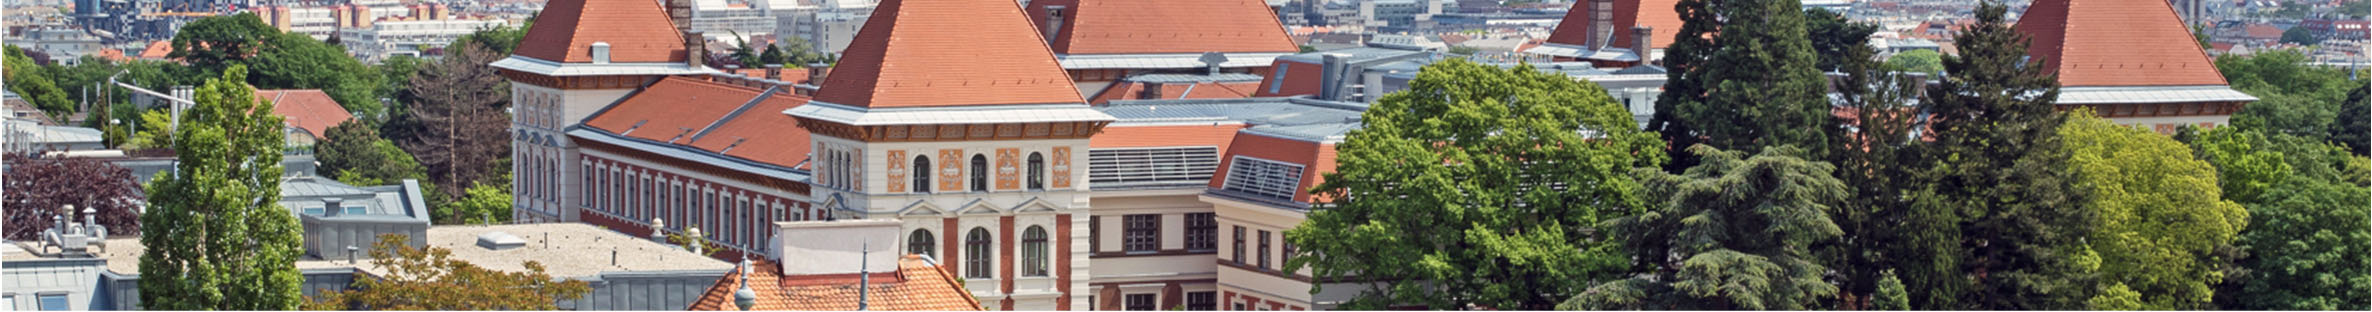
\includegraphics[width=\paperwidth]{_images/boku_header_lower.png}}
    \begin{frame}[c, plain, noframenumbering]{}
        % \centering
        \begin{center}%
            \LARGE%
            #1
        \end{center}
    \end{frame}
\usebackgroundtemplate{}}

\newcommand{\equationBox}[2]{%
    \begin{block}{#1}%
        \vspace*{-2em}\setlength\belowdisplayshortskip{0pt}%
        #2%
        \vspace*{-2em}\setlength\belowdisplayshortskip{0pt}%
\end{block}}

\DeclareCiteCommand{\fullcite}
{\usebibmacro{prenote}}
{\clearfield{url}%
    \clearfield{pages}%
    \clearfield{pagetotal}%
    \clearfield{edition}%
    \clearfield{doi}%
    \clearfield{labelyear}%
    \usedriver
    {\DeclareNameAlias{sortname}{default}}
{\thefield{entrytype}}}
{\multicitedelim}
{\usebibmacro{postnote}}

\DeclareCiteCommand{\fullcitesmall}
{\small\usebibmacro{prenote}}
{\clearfield{url}%
    \clearfield{pages}%
    \clearfield{pagetotal}%
    \clearfield{edition}%
    \clearfield{doi}%
    \clearfield{labelyear}%
    \usedriver
    {\DeclareNameAlias{sortname}{default}}
{\thefield{entrytype}}}
{\multicitedelim}
{\usebibmacro{postnote}}

\DeclareFieldFormat{bibqrcode}{\qrcode[height=1cm]{\thefield{url}}}

\DeclareCiteCommand{\citeqrcode}{%
  \boolfalse{citetracker}%
  \boolfalse{pagetracker}%
  \usebibmacro{prenote}%
}{%
  \printfield[bibqrcode]{url}%
}{%
  \multicitedelim
}{%
  \usebibmacro{postnote}%
}%



\renewcommand{\*}{\mathrm}


\newcommand{\overlayQRCode}[1]{%
    \begin{tikzpicture}[remember picture, overlay]
\node [inner sep=0pt,]
    at (current page.center) {\includegraphics[width=1cm]{#1}};
\end{tikzpicture}
}

\begin{document}

\begin{frame}[plain]
    \titlepage
\end{frame}
% \addtocounter{framenumber}{-1}
% \usebackgroundtemplate{}}

%\section{Section 1}
%\sectionFrame{Part I -- Introduction}


%\begin{frame}
%    \vspace*{1cm plus 1fil}
%    \tableofcontents
%    \vspace*{0cm plus 1fil}
%\end{frame}

%\begin{frame}[t]
%    \frametitle{Frametitle}
%    \only<1|handout:1>{%
%    \centering%
%    \begin{itemize}
%        \item itemize
%        \begin{itemize}
%            \item[\Rightarrow] itemize ...
%        \end{itemize}
%    \end{itemize}
%    \begin{figure}
%        \centering
%        
\includegraphics[width=0.5\linewidth]{template/_images/BOKU_Hauptlogo_CMYK.pdf}
%        \caption{template figure}
%        \label{fig:template}
%    \end{figure}
%    }
%\end{frame}
%
\begin{frame}
\frametitle{Introduction}
   \textbf{Itemized lists:}
   \begin{itemize}
      \item Level 1
      \begin{itemize}
         \item Level 2
         \begin{itemize}
            \item Level 3
         \end{itemize}
      \end{itemize}
   \end{itemize}

\bigskip

   \textbf{Enumerated lists:}
   \begin{enumerate}
      \item First item
      \item Second item
      \item Third item
   \end{enumerate}

\end{frame}
%
\begin{frame}[fragile]
\frametitle{Formatting}

   \textbf{Highlighting:} \textbf{bold}, \textit{italic}, {\color{bokugreen} BOKU green}, {\color{bokuorange} BOKU orange}, \dots

   \bigskip
   
   \textbf{Predefined colors:}
   
   \smallskip
   
   \fcolorbox{black}{bokugreen}{\rule{0pt}{.6em}\rule{.5em}{0pt}} \quad green (\verb|bokugreen|) \\[1mm]
   \fcolorbox{black}{bokugreenl}{\rule{0pt}{.6em}\rule{.5em}{0pt}} \quad light green (\verb|bokugreenl|) \\[1mm]
   \fcolorbox{black}{bokuorange}{\rule{0pt}{.6em}\rule{.5em}{0pt}} \quad orange (\verb|bokuorange|) \\[1mm]
   \fcolorbox{black}{bokuorangel}{\rule{0pt}{.6em}\rule{.5em}{0pt}} \quad light orange (\verb|bokuorangel|) \\[1mm]
   \fcolorbox{black}{bokupurple}{\rule{0pt}{.6em}\rule{.5em}{0pt}} \quad purple (\verb|bokupurple|) \\[1mm]
   \fcolorbox{black}{bokupurplel}{\rule{0pt}{.6em}\rule{.5em}{0pt}} \quad light purple (\verb|bokupurplel|) \\[1mm]
   \fcolorbox{black}{bokugray}{\rule{0pt}{.6em}\rule{.5em}{0pt}} \quad gray (\verb|bokugray|) \\[1mm]
   \fcolorbox{black}{bokugraym}{\rule{0pt}{.6em}\rule{.5em}{0pt}} \quad medium gray (\verb|bokugraym|) \\[1mm]
   \fcolorbox{black}{bokugrayl}{\rule{0pt}{.6em}\rule{.5em}{0pt}} \quad light gray (\verb|bokugrayl|)

\end{frame}
%
\begin{frame}[fragile]
\frametitle{Beamer blocks}

   \begin{block}{Block}
      This is a block.

      Uses \verb|bokugreen| and \verb|bokugreenl|.
   \end{block}

\medskip

   \begin{alertblock}{Alert block}
      This is an alert block.

      Uses \verb|bokuorange| and \verb|bokuorangel|.
   \end{alertblock}

\medskip

   \begin{exampleblock}{Example block}
      This is an example block.

      Uses \verb|bokupurple| and \verb|bokupurplel|.
   \end{exampleblock}

\end{frame}
%
%\begin{frame}[t]
%    \frametitle{build itemize}
%    \begin{minipage}[t][\textheight-2\fboxsep-2\fboxrule][t]{0.65\textwidth}%
%        \textbf{template point}:
%        \begin{itemize}
%            \item<1-> item 1
%            \item<2-> item 2
%            \item<3-> item 3
%                \begin{itemize}
%                    \item[-]<3-> subitem 3.1
%                    \item[-]<4-> subitem 3.2
%                \end{itemize}
%            \item<5-> item 4
%        \end{itemize}
%    \end{minipage}%
%    \hfill%
%\end{frame}

\title[Template]{Thanks!}
\subtitle{}

\begin{frame}[plain]
    \begin{tikzpicture}[remember picture,overlay,anchor=north west,inner sep=0pt]
        \node[xshift=2.5mm,yshift=-2.5mm] at (current page.north west) {
    	   
\includegraphics[width=32.1mm]{template/_images/BOKU_Hauptlogo_CMYK.pdf}%
        };
    \end{tikzpicture}
    \titlepage
\end{frame}

\end{document}

